% Copyright � 2015 by James Dean Mathias
% All Rights Reserved

\chapter{Scalability - Distributed}\label{chapter:dist}

Some problems require more computing resources than are reasonably available on a single system. The scale and/or timing constraints of these problems force the need to bring together a number of networked systems and distribute the computing tasks among them; hence the term \textit{distributed computing}. This chapter tackles the biggest change to the scalability framework, distributing tasks to other computers and returning the results.

In order to distribute tasks over multiple systems, two fundamental changes are required to the framework. The first and most obvious is that two different kinds processes are necessary, separate client and server processes. The second is that of a networking framework through which messages are sent and received. While the framework continues to be familiar, these are big changes and require the addition a lot of new code.

A secondary change is with respect to building the system. These changes result in three separate projects, shared code, client code, and server code. The client and server share a large amount of code in commmon, therefore most of the system code is in a shared project that is compiled to a static library and linked into both the client and server projects. The client and server each have a smaller set of code that make them unique, two projects are created that buidl the separate processes.

% Discuss using of thread pools on io\_service (at the distributer) and strands

\section{System Design}\label{chapter:dist:design}

The system design approach presented in this chapter, and the next two, is that of a single interactive client and many connected compute servers; \FigureGeneral \ref{chapter:dist:design} illustrates this design. In our case, the client is the interactive Mandelbrot application. The client generates computational tasks in response to the user changing the view. These tasks are distributed among the servers. The servers receive tasks, execute them, and return the results back to the client.

% Source: http://tex.stackexchange.com/questions/15731/tikz-task-diagram-alignment-and-arrows
\begin{figure}
	\centering
	\begin{tikzpicture}[rounded corners=2pt,inner sep=5pt,node distance=2.0cm]
		\node [draw](client) { \textit{Client}};
		\node [inner sep=0pt, below=of client](aux) {\strut};
		\node [draw,left=.7cm of aux] (server2) {\textit{Server$_2$}};
		\node [draw,right=.7cm of aux] (server3) {\textit{Server$_{\ldots}$}};
		\node [draw,left=of server2] (server1) {\textit{Server$_1$}};
		\node [draw,right=of server3] (server4) {\textit{Server$_n$}};
		\foreach \n in {1,...,4}
			\draw [<->] (client) -- (server\n.north);
	\end{tikzpicture}
	\caption{System Design}\label{chapter:dist:design}
\end{figure}

The use of the terms \textit{client} and \textit{server} may sound a little different than what you may expect, but they aren't. A typical description of a system is that of a server with many connected clients, for example many web browsers and a single web server. In the model presented in this chapter, there is a single client, but many connected servers. If you think about the clients and servers, regardless of their number, they perform the same roles in both models. In the case of the clients, a web server or an interactive Mandelbrot application, they both respond to user inputs and make requests to a server, or servers. With respect to a server in a web system, the web server receives requests, performs computational tasks and returns those results to the client. The server in our system receives tasks, executes those tasks, and returns the results to the client. In other words, the use of the terms is the same, it is only the system topology that is different.

\FigureGeneral \ref{chapter:dist:model-figure} provides an overview of the system model. The client process accepts input from the user and generates compute tasks, it is the server(s) that perform the execution of the tasks. Rather than tasks being placed into a client thread pool as is done in the previous chapters, tasks are placed into a \textit{Global Task Queue} from which they are distributed throughout the connected compute servers. Immediately after making a successful connection, a compute server sends a set of task requests to the client (represented by the arrow from the compute server to the \textit{Task Request Queue}), indicating it is available to receive work. The \textit{Task Request Queue} holds the requests from the servers which get matches with waiting tasks. When a match is made, the task is transmitted to the compute server and placed in its \textit{Local Task Queue} (represented by the arrow from the client \textit{Global Task Queue} to the compute server \textit{Local Task Queue}) from which the server selects, executes the tasks, compiles the results, and returns the results back to the client.

\begin{figure}[H]
	\centering	
	\fbox
	{
		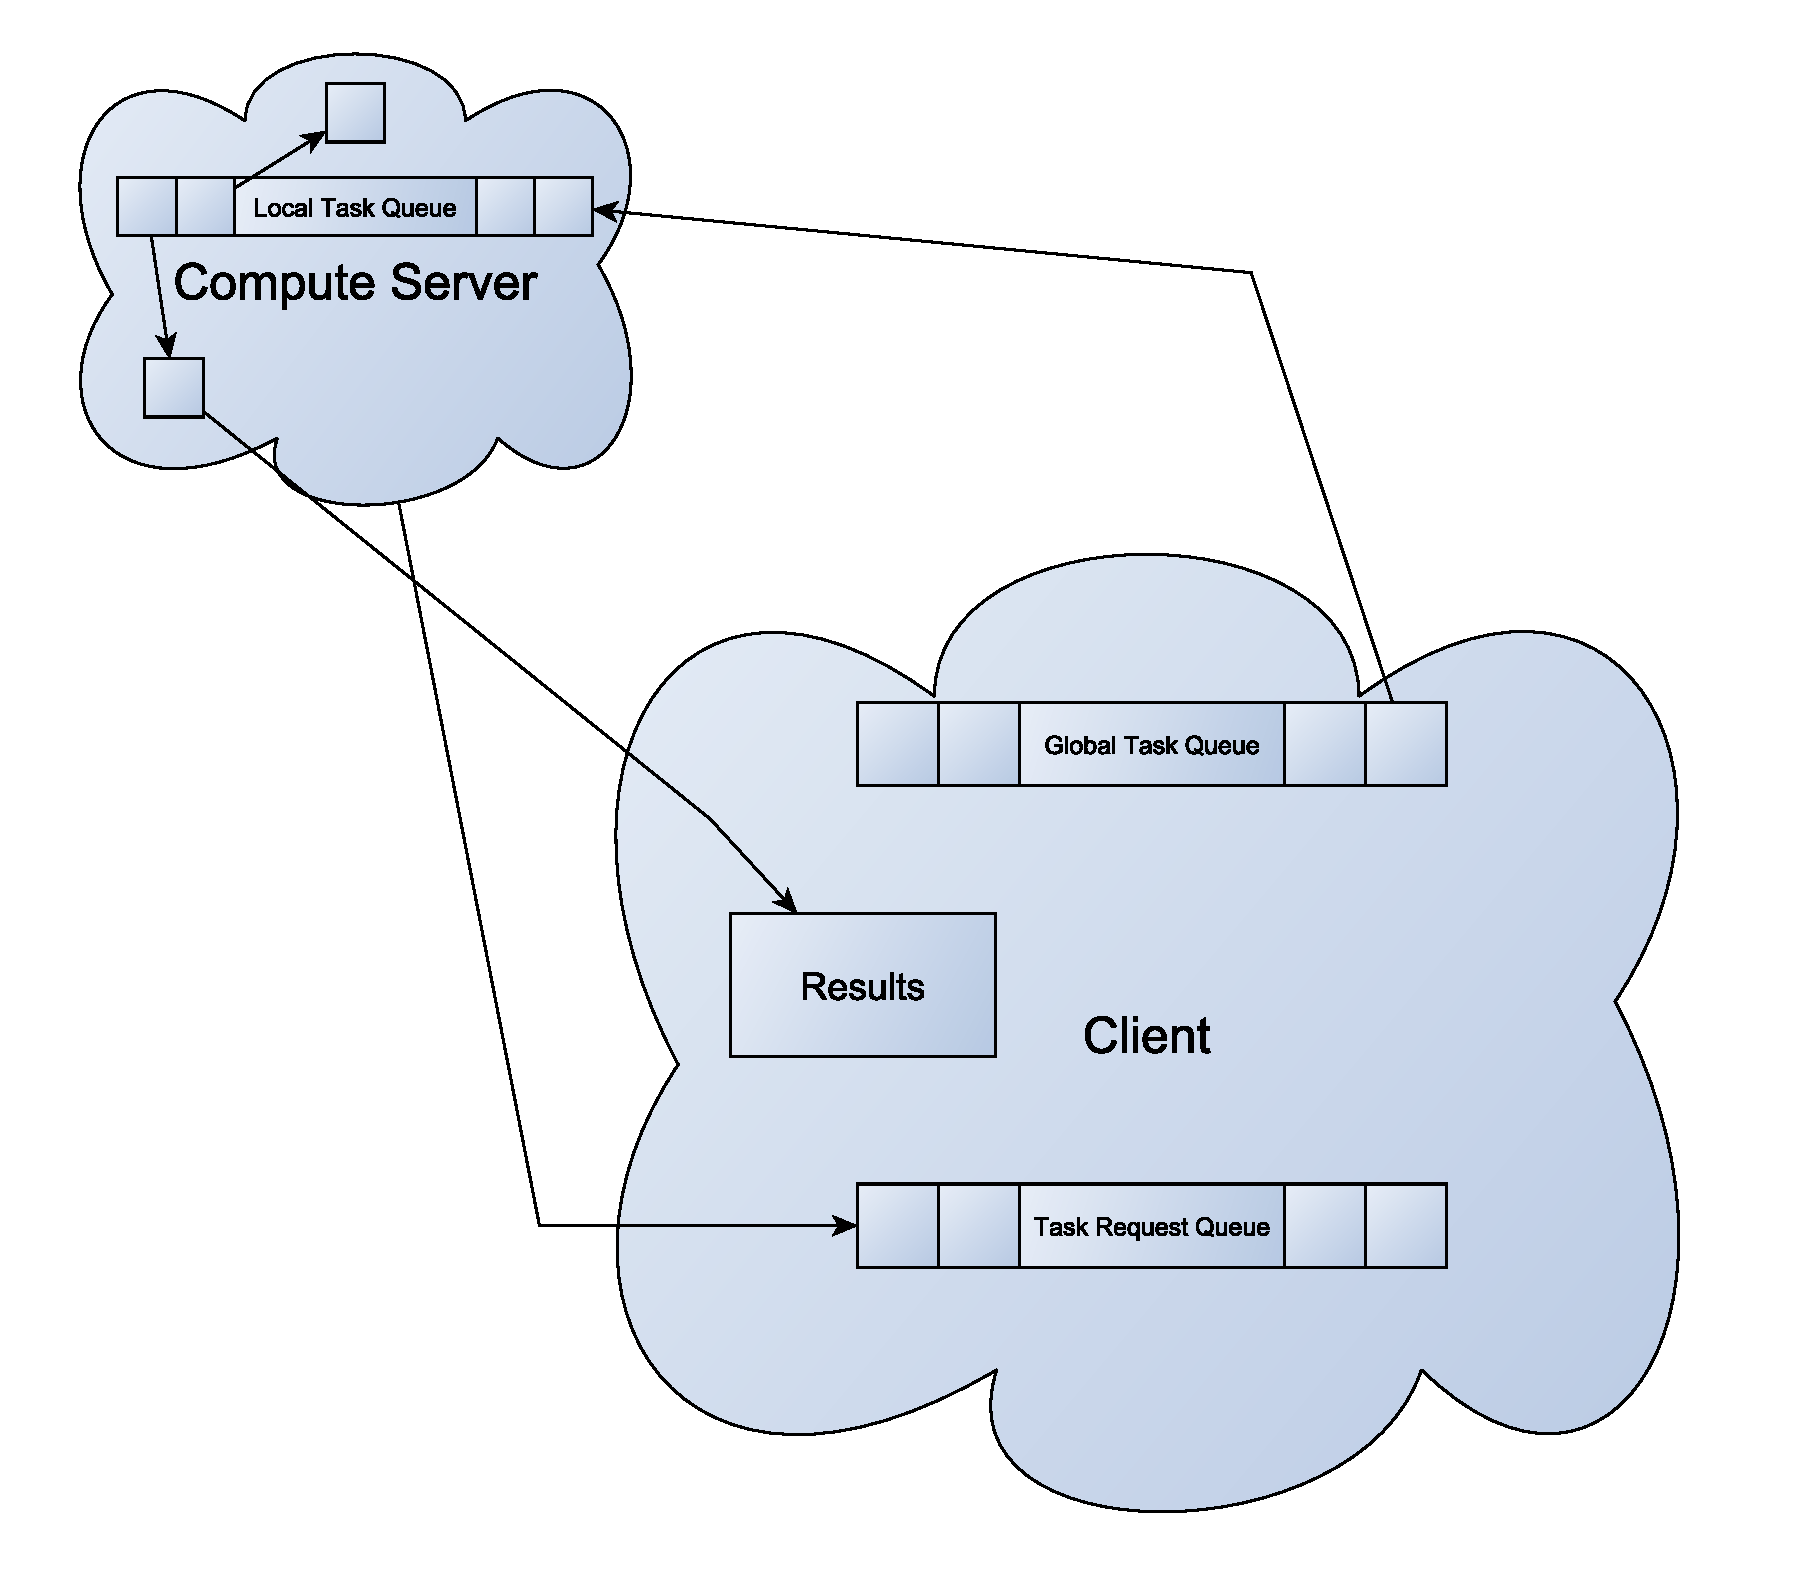
\includegraphics[width=4.5in, height=4.5in]{Images/Distributed-Model.pdf}
	}
	\caption{Distributed Model}
	\label{chapter:dist:model-figure}
\end{figure}

The small squares with arrows pointing to them on the compute server represent tasks that have been removed from the \textit{Local Task Queue} and are being executed. The arrow going from the small square on the compute server to the \textit{Results} box represents a task that has finished execution and its results being sent back to the client.

The model in this figure is only that, a model, the implementation details have additional complexity. The specifics of how this model is implemented are presented in the remainder of the chapter.

\FigureGeneral \ref{chapter:dist:communication-figure} shows the sequence of communication that takes place between the client and a server. The first step is for a server to initiate and establish a connection with the client. Upon successful connection, the server then sends a task request to the client, indicating it is available to perform work. When the client is ready to have a task computed, it sends a task to the server, the server computes the result, sends it back to the client, and immediately sends another task request indicating it can take on more work with the completion of the previous task. In the case the client is shutting down, it sends a termination message to all connected servers instructing them to gracefully shutdown.

\begin{figure}[H]
	\centering	
	\includegraphics[width=4.5in, height=4.5in]{Images/Distributed-Communication-Sequence.png}
	\caption{Distributed Communication}
	\label{chapter:dist:communication-figure}
\end{figure}

Not shown in this diagram, but implied, is once the client receives the results, it places them into the display buffer for immediate viewing; or in the case of a prime number, reports the result to the console upon receipt.

The core fundamental continues to hold true, decomposing a problem into computable tasks. The compute servers indicate their availability for work, ensuring the client only sends a task when it has available resources. Because of this, the system as a whole continues to exhibit a scalable nature by automatically load balancing the tasks over the connected compute servers. Because of the design and implementation groundwork laid in the first version of the application, all of the major components that ensure scalability are already in place, significantly easing the transition to a distributed framework, while maintaining the scalable nature.

\section{Networking Infrastructure} %Shared

Chapter \ref{chapter:networking} introduced the networking techniques used as the basic building blocks for distributed communication. The discussion was furthered in Chapter \ref{chapter:coding} with a description of how messages are coded and encoded for transmission between processes. This section continues the discussion by futher detailing the networking framework.

\subsection{Client \& Server Initialization}

The code presented in the previous chapters placed the basic application framework in a class named \texttt{ScalabilityApp}, the code associated with this chapter renames the class to \texttt{DistributedApp} to better reflect its nature. In addition to a new name, quite a bit of new code has been added. One of these new additions is the initialization of the Boost.Asio library's \texttt{io\_service}. This code is contained in the \texttt{DistributedApp::initialize} method, shown in \FigureCode \ref{chapter:dist:client-initialize}. Remember that the system is now composed of two processes, a client and server, this code is only part of the client process.

\begin{code}[caption={Client Initialization}, label=chapter:dist:client-initialize]
bool DistributedApp::initialize()
{
  using namespace boost::asio;
  m_threadWork = std::unique_ptr<io_service::work>
    (new io_service::work(m_ioService));
  for (auto thread : IRange<uint8_t>(1, 10))
  {
    m_threadsIO.push_back(std::unique_ptr<std::thread>(
      new std::thread(
        [this]()
        {
          m_ioService.run();
        })));
  }

  TaskRequestQueue::instance()->initialize(&m_ioService, &m_servers);

  waitOnConnection();

  return true;
}
\end{code}

The first part of this function creates the \texttt{io\_service}, along with assigning a pool of threads. The client will have potentially many connected compute servers, this allows many different connections to be serviced concurrently. An \texttt{io\_service::work} object is also created and associated with the \texttt{io\_service} to prevent it from terminating when there are no events on its request queue. The next step is to initialize the \texttt{TaskRequestQueue}, which needs to have access to the application \texttt{io\_service}; this singleton is fully discussed in Section \ref{chapter:dist:client}. The final step in the initialization is to begin waiting for connections from servers, which is described in the next section.

The server has an analogous initialization to the client, shown by the two code sections in \FigureCode \ref{chapter:dist:server-initialize}. It creates an \texttt{io\_service} queue, \texttt{io\_service::work} object, but only places a single thread on the \texttt{io\_service}. The server only ever communicates with the client, therefore the need to have more than one thread to handle network communication is not necessary. Following this, an instance of a class named \texttt{ComputeServer} is created and initialized. During its initialization a familiar \texttt{ThreadPool} is initialized, from which assigned tasks are associated and executed. Finally, the server enters a state where it initiates a connection to the client, this procedure is discussed in the next section.

\begin{code}[caption={Server Initialization}, label=chapter:dist:server-initialize]
int main(int argc, char* argv[])
{
  ...
  boost::asio::io_service ioService;
  boost::asio::io_service::work work(ioService);

  std::thread thread = std::thread(
    [&ioService]() 
    { 
        ioService.run();
    });

  ComputeServer server;
  server.initialize(ioService, ipClient, portClient);
  ...
}

void ComputeServer::initialize(
  boost::asio::io_service& ioService, 
  const std::string& ipClient, 
  const std::string& portClient)
{
  ThreadPool::instance()->initialize(&ioService);
  connectToClient(ioService, ipClient, portClient);
}
\end{code}

\subsection{Making a Connection}

Section \ref{chapter:networking:sockets:connection} of Chapter \ref{chapter:networking} provides the background on how to use Boost.Asio to initiate and accept networking connections. The code presented in this chapter follows those techniques, with a few minor differences owing to the context of the Mandelbrot viewing application.

The connection model used by the Mandelbrot application is to have the client wait for an incoming connection from a compute server. For the approach used in the Mandelbrot application, the servers must know the location of the client, but the client does not need advance knowledge of the servers. The start order of the processes doesn't matter. Upon start, a compute server continues to attempt making a connection to the client, retrying until either the connection is established or the process is manually terminated. Similarly, upon start, the client begins waiting for incoming connections, and allowing them to be made at any time during the application lifetime, not only during an initialization phase. This allows the client to take advantage of ever more computing resources over time. The code presented in this chapter does not discuss how to handle servers that disconnect or fail while the client is alive; a topic complex enough to require its own discussion, and tackled in Chapter \ref{chapter:ft}.

The server code for initiating a connection with the client is found in \FigureCode \ref{chapter:dist:init-connect}. The first part of the method is almost exactly as found in Section \ref{chapter:networking:init-connection} of Chapter \ref{chapter:networking}. The one difference is the use of the blocking \texttt{connect} instead of the non-blocking \texttt{async\_connect}. The reason for this is that the server doesn't need to do anything else while waiting for the connection to complete, therefore, the code is simplified by using a blocking call.

\begin{code}[caption={Initiating A Connection}, label=chapter:dist:init-connect]
void ComputeServer::connectToClient(
  boost::asio::io_service& ioService, 
  const std::string& ipClient, 
  const std::string& portClient)
{
  ip::tcp::resolver resolver(ioService);
  ip::tcp::resolver::query query(ipClient, portClient);
  ip::tcp::resolver::iterator iterator = resolver.resolve(query);

  bool done = false;
  while (!done)
  {
    auto socket = std::make_shared<tcp::socket>(ioService);
    boost::system::error_code error;
    boost::asio::connect(*socket, iterator, error);
    if (!error)
    {
      done = true;
      waitOnTask(socket);
      unsigned int count = std::max(
        1u, 
        std::thread::hardware_concurrency()) * 2;
      for (auto core : IRange<unsigned int>(1, count))
      {
        ioService.post(
          [socket]()
          {
            Messages::TaskRequest command;
            command.send(socket);
          });
      }
    }
  }
}
\end{code}

Once the \texttt{connect} method returns without error, \texttt{done} is set to \texttt{true} to indicate a successful connection has been made and the connection loop can end. Next, a call to the non-blocking \texttt{waitOnTask} method is made. This method, detailed in Section \ref{chapter:dist:network:receive-messages}, waits for task messages from the client. The final step is to send a number of task requests to the client. Each request indicates the availability of enough resources to compute one task. This is done by creating a bunch of \texttt{TaskRequest} messages and sending them over the connected socket.

The reason for sending more task requests than the number of available cores is to allow for I/O operations to be taking place while other tasks are executing. Consider that a system can be sending a task request, receiving a task, sending the results from executing a task, and executing several other tasks, all at the same time. On the other hand, only a single thread is assigned to the \texttt{io\_service}, for a number of reasons. Foremost is that there is only one network card, and only one connection to a single client. Secondly, the expectation with the server is for it to be compute bound, working on tasks, instead of being I/O bound, sending and receving messages over the network. Time spent computing should dominate the time spent performing I/O, if at all possible. In order to more effectively keep the CPU cores fully utilized, it is necessary to have at least one task waiting for execution as soon as one completes. This means the number of task requests must exceed the number of available CPU cores by enough to prevent the system from waiting for I/O to complete to begin execution of the next task.

The other side of the connection is the client, which waits for an incoming connection request; the code shown in \FigureCode \ref{chapter:dist:wait-connect} demonstrates this. Again, the code for the client follows the pattern described in Section \ref{chapter:networking:accept-connection} of Chapter \ref{chapter:networking}. When a successful a connection is made, a \texttt{Server} instance is created and added to the list of known servers. This is followed by a call to the non-blocking method \texttt{waitOnMessage}, described in Section \ref{chapter:dist:network:receive-messages}.

\begin{code}[caption={Waiting For Connection}, label=chapter:dist:wait-connect]
void DistributedApp::waitOnConnection()
{
  auto socket = std::make_shared<ip::tcp::socket>(m_ioService);
  m_acceptor.async_accept(*socket,
    [this, socket](const boost::system::error_code& error)
    {
      if (!error)
      {
        Server server(socket);
        m_servers.add(server);
        waitOnMessage(server.id);
      }
      waitOnConnection();
  });
}
\end{code}

The \texttt{Server} struct is used by the client to maintain connection information about a connected server. Each instance is also assigned a unique identifier that is used as the key for reference in a hash table in the \texttt{ServerSet} class. The struct also holds a pointer to the socket over which communication takes place. In order to ensure valid synchronization of threads communicating with each server, as described in Chapter \ref{chapter:networking}, each server is given its own \texttt{strand}; all communication requests with the server are posted to this \texttt{strand}. The code for this struct is found in \FigureCode \ref{chapter:dist:server-struct}.

\begin{code}[caption={\texttt{Server} Struct}, label=chapter:dist:server-struct]
struct Server
{
  Server() {} 
  Server(boost::asio::io_service& ioService)
  {
    static ServerID_t newId = 0;
    this->id = newId++;
    this->strand = std::make_shared<boost::asio::strand>(
        socket->get_io_service());
  }

  ServerID_t id;
  std::shared_ptr<ip::tcp::socket> socket;
  std::shared_ptr<boost::asio::strand> strand;
  std::array<uint8_t, 1> messageType;
};
\end{code}

Associated with the \texttt{Server} struct is a class named \texttt{ServerSet} which is used as a container to maintain details of all connected servers. This class primarily provides synchronized access to the list of available servers. The \texttt{add}, \texttt{get}, and \texttt{exists} are simple helper methods that control, and synchronize, access to the \texttt{std::unordered\_map} of \texttt{Server} structs. The declaration for this class is shown in \FigureCode \ref{chapter:dist:server-set}.

\begin{code}[caption={\texttt{ServerSet} Class}, label=chapter:dist:server-set]
class ServerSet
{
public:
  void add(Server server);
  boost::optional<Server&> get(ServerID_t id);
  bool exists(ServerID_t id);
  std::unordered_map<ServerID_t, Server> getServers();

private:
  std::unordered_map<ServerID_t, Server> m_servers;
  std::mutex m_mutex;
};
\end{code}

\subsection{Command Pattern}\label{chapter:dist:network:command-pattern}

This distributed application takes advantage of a design pattern known as the \textit{Command Pattern}\footnote{http://en.wikipedia.org/wiki/Command\_pattern} to reduce code complexity and improve it for future maintenance, as additional messages are added to the system. The design pattern is used to associate a message type with a handler function or method. The implementation uses a hash table (\texttt{std::unordered\_map}), where a message type is used as the key and the value is a \texttt{std::function}; which is invoked when the message type is received. The hash table type for the client is shown in \FigureCode \ref{chapter:dist:client-pattern-type}, and the server type is shown in \FigureCode \ref{chapter:dist:server-pattern-type}.

\begin{code}[caption={Client Command Pattern Type}, label=chapter:dist:client-pattern-type]
std::unordered_map<
  Messages::Type, 
  std::function<void (ServerID_t)>>
\end{code}

\begin{code}[caption={Server Command Pattern Type}, label=chapter:dist:server-pattern-type]
std::unordered_map<
  Messages::Type, 
  std::function<void (std::shared_ptr<ip::tcp::socket>)>>
\end{code}

For the client, the function handler accecpts a \texttt{ServerID\_t} as a parameter, which is the unique identifier for the server from which the message originated. This parameter is then used to lookup the server from the \texttt{ServerSet} and retrieve the socket connection for communication. For the server, the function handler accepts the socket over which communication to the client takes place. There is only one socket between the server and client, therefore no need to manage and lookup different sockets for different routes of communication at the server.

The client and server both declare a member variable named \texttt{m\_messageCommand} of their command pattern types in the \texttt{DistributedApp} and \texttt{ComputeServer} classes, respectively; I refer to these as \textit{command maps}. During application initialization, the command maps are initialized with the different types of messages that can be received and their associated handlers. The initialization code for the client is show in \FigureCode \ref{chapter:dist:client-pattern-init}.

\begin{code}[caption={Client Command Map Initialization}, label=chapter:dist:client-pattern-init]
void DistributedApp::prepareCommandMap()
{
  m_messageCommand[Messages::Type::TaskRequest] = 
    [this](ServerID_t serverId) 
    { 
      processTaskRequest(serverId); 
    };
  m_messageCommand[Messages::Type::MandelResult] = 
    [this](ServerID_t serverId) 
    { 
      processMandelResult(serverId); 
    };
  m_messageCommand[Messages::Type::NextPrimeResult] = 
    [this](ServerID_t serverId) 
    { 
      processNextPrimeResult(serverId); 
    };
}
\end{code}

The \texttt{prepareCommandMap} method associates a lambda function with each of the types of messages it may receive from a compute server. The lambda has the same signature as the \texttt{std::function} defined as part of the \texttt{m\_messageCommand} type. Upon invocation, the lambda simply makes a call to an instance method that performs the actual work of handling the message type. The initialization of the command map for the server looks the same as the client, except that it responds to different message types and invokes different handlers.

The code in \FigureCode \ref{chapter:dist:pattern-sample} demonstrates how to use the command map to invoke the handler for a specific message. The \texttt{[Messages::Type::TaskRequest]} part of the statement searches the hash table for the entry corresponding to that key, which is a function. Then, the \texttt{(serverId)} part of the statement invokes the returned function.

\begin{code}[caption={Command Map Invocation}, label=chapter:dist:pattern-sample]
m_messageCommand[Messages::Type::TaskRequest](serverId);
\end{code}

There command map code for the server is able to be somewhat simplified over the client code because the same thing is done for all messages except for one. Because of this, the code for the server can take advantage of generic programming by having a templated \texttt{processTask} function that does the same thing for every message and task type combination. The code for this function is shown in \FigureCode \ref{chapter:dist:server-processtask}. This function simply reads the remainder of the message from the socket, then places the task onto the local \texttt{ThreadPool} for execution.

\begin{code}[caption={Server Templated \texttt{processTask}}, label=chapter:dist:server-processtask]
template <typename Message, typename Task>
void processTask(std::shared_ptr<ip::tcp::socket> socket)
{
  Message message;
  message.read(socket);
  std::shared_ptr<Tasks::Task> task = std::make_shared<Task>(socket, message);

  ThreadPool::instance()->enqueueTask(task);
}
\end{code}

The initialization of the server command map makes use of the templated \texttt{processTask} function. As this method is used, the message and task types are specified as template parameters for the \texttt{processTask} function, as demonstrated in \FigureCode \ref{chapter:dist:server-pattern-init}. There is one exception to the messages received at the server, and that is the terminate command. A \texttt{TerminateCommand} message is not a computational task, therefore it doesn't belong on the \texttt{ThreadPool}, it is a message instructing the server process to perform a graceful shutdown. Because of this, a specific function is used to handle that message, \texttt{processTerminateCommand}, which is reflected in the initialization of the command map.

\begin{code}[caption={Server Command Map Initialization}, label=chapter:dist:server-pattern-init]
void ComputeServer::prepareCommandMap()
{
  m_messageCommand[Messages::Type::MandelMessage] = 
    [this](std::shared_ptr<ip::tcp::socket> socket)
    {
      processTask<Messages::MandelMessage, Tasks::MandelTask>(socket);
    };
  m_messageCommand[Messages::Type::NextPrimeMessage] = 
    [this](std::shared_ptr<ip::tcp::socket> socket)
    {
      processTask<Messages::NextPrimeMessage, Tasks::NextPrimeTask>(socket);
    };
  m_messageCommand[Messages::Type::TerminateCommand] =
    [this](std::shared_ptr<ip::tcp::socket> socket)
    {
      processTerminateCommand(socket);
    };
}
\end{code}

\subsection{Receiving Messages}\label{chapter:dist:network:receive-messages}

The technique for message encoding before sending was presented in Chapter \ref{chapter:coding}, along with how a message is read and decoded once the message type is known. But we still need to understand how an application waits for messages to arrive, determines the message type in order to create the correct message instance, and then passed off to be read and decoded.

\FigureCode \ref{chapter:dist:client:wait-message} shows the \texttt{waitOnMessage} that is called whenever a compute server makes a connection to the client. Almost all of the code is a lambda that is passed as a parameter to the non-blocking \texttt{async\_receive} call. This becomes a handler on the \texttt{io\_service} that is invoked whenever a message is received over this socket. Think carefully about this, for each connected server there is a pending receive handler associated with the socket connection; it is not a single handler for all servers, it is multiple handlers, one for each connected server/socket.

\begin{code}[caption={Client \texttt{waitOnMessage}}, label=chapter:dist:client:wait-message]
void DistributedApp::waitOnMessage(ServerID_t serverId)
{
  boost::optional<Server&> server = m_servers.get(serverId);
  server->socket->async_receive(boost::asio::buffer(server->messageType),
    [this, serverId, server]
    (const boost::system::error_code& error, std::size_t bytes)
    {
      if (!error && bytes > 0)
      {
        Messages::Type type = 
          static_cast<Messages::Type>(server->messageType[0]);
        m_messageCommand[type](serverId);
        waitOnMessage(serverId);
      }
    });
}
\end{code}

The \texttt{Server} structure defines a single byte \texttt{std::array} that is used as a buffer into which the first byte of a message is received. This array is passed as the first parameter to the \texttt{async\_recieve} call. The second parameter is the lambda to invoke when the byte is received. Section \ref{chapter:coding:send-receive} of Chapter \ref{chapter:coding} showed that the first byte sent as part of a message is the unique message type. The client can receive three different messages from the server: a request for a task, results for a Mandelbrot task, and the results from a prime number task. These three messages correspond to the following enumeration types: \texttt{Messages:Type::TaskRequest}, \texttt{Messages::Type::MandelResult}, \texttt{Messages::Type::NextPrimeResult}. These are the three message handlers registered with the command map presented in Section \ref{chapter:dist:network:command-pattern}.

As a bit of sanity checking, the first part of the lambda checks to see if an error occurred on the socket, causing the handler to be invoked. If no error occurred, the rest of the message is processed. The next bit of code casts the received byte to a \texttt{Messages::Type} allowing it to be used as the key for invoking the message handler on the \texttt{m\_messageCommand} hash table. It is during the this call that the rest of the message is read from the socket, decoded, and processed. Once the call on the command map has completed, a new call to \texttt{waitOnMessage} is made in order to place a new handler on the \texttt{io\_service} to respond the next message received.

An example command map handler is shown in \FigureCode \ref{chapter:dist:client:process-prime}. This method is invoked when a prime number result message is received from a compute server. The lambda registered in the \texttt{waitOnMessage} reads the first byte of the message, then based upon that message, this handler is invoked. This handler creates an instance of the \texttt{NextPrimeResultMessage} class, which then finishes reading the data from the socket and decodes the results into the class members.

\begin{code}[caption={Process Prime Result}, label=chapter:dist:client:process-prime]
void DistributedApp::processNextPrimeResult(
    ServerID_t serverId)
{
  Messages::NextPrimeResultMessage taskResult;
  taskResult.read(m_servers.get(serverId)->socket);

  m_lastPrime = taskResult.getNextPrime();
  m_reportPrime = true;
  std::shared_ptr<Tasks::NextPrimeTask> task = 
    std::make_shared<Tasks::NextPrimeTask>(
      taskResult.getNextPrime(), 
      Tasks::Task::Priority::Three);
  TaskRequestQueue::instance()->enqueueTask(task);
}
\end{code}

With the result message processed, the handler remembers the newly generated prime number to the private class member \texttt{m\_lastPrime}. Next, the \texttt{m\_reportPrime} boolean is set to \texttt{true}, which tells the application to display the \texttt{m\_lastPrime} value to the console. Finally, a new \texttt{NextPrimeTask} is created and placed on the \texttt{TaskRequestQueue}. This function completes the prime number computation loop, keeping the computation ongoing throughout the lifetime of the application.

The compute server is substantially similar to the client. It makes a call to the non-blocking \texttt{async\_receive}, passing a single byte buffer as the first parameter and a lambda to be invoked upon receipt of the byte. Once again, the byte is converted to a \texttt{Messages::Type}, the command map handler invoked, and then a new call to \texttt{waitOnTask} is made. The code for this method is found in \FigureCode \ref{chapter:dist:server:wait-task}.

\begin{code}[caption={Server \texttt{waitOnTask}}, label=chapter:dist:server:wait-task]
void ComputeServer::waitOnTask(
    std::shared_ptr<ip::tcp::socket> socket)
{
  socket->async_receive(boost::asio::buffer(m_messageType),
    [this, socket](const boost::system::error_code& error, std::size_t bytes)
    {
      if (!error)
      {
        Messages::Type type = static_cast<Messages::Type>(m_messageType[0]);
        m_messageCommand[type](socket);
        waitOnTask(socket);
      }
    });
}
\end{code}

\subsection{Sending Tasks}\label{chapter:dist:network:send-task}

The \texttt{Task} is updated to reflect the nature of a distributed application. A task now knows how to send itself to a compute server via a socket, along with knowing how to return a computed result back to the client. These new capabilities have changed the application interface through the addition of a new \texttt{send} method, and a change in the approach to how the \texttt{complete} method is implemented. \FigureCode \ref{chapter:dist:task-decl} shows a portion of the revised \texttt{Task} class delcaration.

\begin{code}[caption={Revised \texttt{Task} Declaration}, label=chapter:dist:task-decl]
class Task
{
public:
  void send(
    std::shared_ptr<ip::tcp::socket> socket, 
    boost::asio::strand& strand);

  void complete(boost::asio::io_service& ioService);

protected:
  virtual std::shared_ptr<Messages::Message> getMessage() = 0;
  virtual void completeCustom(boost::asio::io_service& ioService) = 0;
};
\end{code}

The new \texttt{send} method has the responsibility to send a task message to a connected server, using the socket and strand passed to it. The implementation for this method is almost trivial, as shown in \FigureCode \ref{chapter:dist:task:send}. The first thing the code does is to call into the derived class \texttt{getMessage} method to obtain a fully formed \texttt{Message} that is then sent to the compute server.

\begin{code}[caption={\texttt{Task::send} Implementation}, label=chapter:dist:task:send]
void Task::send(
  std::shared_ptr<ip::tcp::socket> socket, 
  boost::asio::strand& strand)
{
  auto message = getMessage();
  message->send(socket, strand);
}
\end{code}

Notice that \texttt{Task::getMessage} is a pure virtual method, forcing derived \texttt{Task} classes to provide an implementation. The only thing this method needs to do is to construct and return a shared pointer to a \texttt{Message} class that represents the work to be done at the compute server. An example implementation for a \texttt{getMessage} is shown in \FigureCode \ref{chapter:dist:mandel-message:get-message}. The code simply creates and returns a shared pointer to an instance of a \texttt{MandelMessage} using the attribute values of the \texttt{MandelTask} instance.

\begin{code}[caption={\texttt{MandelTask::getMessage} Implementation}, label=chapter:dist:mandel-message:get-message]
std::shared_ptr<Messages::Message> MandelTask::getMessage()
{
  return 
    std::shared_ptr<Messages::MandelMessage>(
      new Messages::MandelMessage(
        m_id, 
        m_startRow, m_endRow, 
        m_sizeX, 
        m_startX, m_startY, 
        m_deltaX, m_deltaY, 
        m_maxIterations));
}
\end{code}

\section{Client Notes}\label{chapter:dist:client}

The client is the Windows part of the distributed application. It is responsible for the display of the Mandelbrot image, along with display of the prime number generation results. In the same way as the previous chapters, the client is responsible for generating the tasks that need to be computed, whether tasks for computing the Mandelbrot set or tasks for computing the next prime number. The difference now is that the client does not contain any code to perform those computations, it only generates the tasks and distributes them to the connected servers. The remainder of this section details how tasks are distributed to the connected servers, along with describing how a graceful shutdown of the client is performed.

\subsection{Matching Tasks \& Requests}

Because the application is now composed of multiple processes, all executing on different computers, it requires a change in how selecting tasks for computation is handled. In the first three versions of the application, tasks were placed on a thread pool. The tasks were then grabbed by an available thread and executed. With the distributed application, the client no longer has that same thread pool, instead, the thread pool is on the server processes, where the tasks are executed. The tasks are generated by the client Mandelbrot application. As described in the first part of the chapter, servers send task requests to the client, and those requests are matched with waiting tasks. This matching takes place on a new singleton object as part of the client, the \texttt{TaskRequestQueue}.

The declaration for the \texttt{TaskRequestQueue} is shown in \FigureCode \ref{chapter:dist:task-request-queue}. This class is immediately familiar because of similarities it shares with the \texttt{ThreadPool}. It is implemented as a singleton, because there should only be one in existence for any application, along with making it globally accessible. Secondly, it has the same \texttt{enqueueTask} method and supporting class members. It diverges in that it is not a thread pool, the addition of the \texttt{enqueueRequest} method, and the distribution algorithm that matches tasks with requests and distributes them to the servers.

\begin{code}[caption={\texttt{TaskRequestQueue} Declaration}, label=chapter:dist:task-request-queue]
class TaskRequestQueue
{
public:
  static std::shared_ptr<TaskRequestQueue> instance();

  void initialize(
    boost::asio::io_service* ioService, 
    ServerSet* servers);
  void terminate();
  void enqueueRequest(ServerID_t request);
  void enqueueTask(std::shared_ptr<Tasks::Task> task);

protected:
  TaskRequestQueue();

private:
  static std::shared_ptr<TaskRequestQueue> m_instance;
  boost::asio::io_service* m_ioService;
  ServerSet* m_servers;

  std::queue<ServerID_t> m_queueRequest;
  std::mutex m_mutexRequest;
  std::condition_variable m_eventRequest;
  std::mutex m_mutexEventRequest;

  ConcurrentPriorityQueue<std::shared_ptr<Tasks::Task>, TaskCompare> m_queueTasks;
  std::condition_variable m_eventTask;
  std::mutex m_mutexEventTask;

  std::shared_ptr<std::thread> m_distributer;
  bool m_distributerDone;

  void distribute();
  void fillRequest(std::shared_ptr<Tasks::Task> task);
};
\end{code}

As indicated in the description above, the \texttt{TaskRequestQueue} has two containers that hold the task requests and tasks. The task requests are stored in the \texttt{m\_queueRequest} member, which is a \texttt{std:queue}. Just like the thread pool from the chapter on priority, the tasks are stored in a new container, a \texttt{ConcurrentPriorityQueue}. This container is a simple thread-safe wrapper around the \texttt{std::priority\_queue}. Each of these containers are associated with a condition variable, \texttt{m\_eventRequest} and \texttt{m\_eventTask} respectively, that are signaled when an item is added.

When the singleton is first used, it creates a private \texttt{m\_distributer} thread. \FigureCode \ref{chapter:dist:trq:instance} shows the \texttt{instance} method where the thread is created. The purpose of this thread is to respond to incoming task requests and tasks, matching and sending them off to be computed. The matching algorithm is discussed later in this section.

\begin{code}[caption={\texttt{TaskRequestQueue::instance}}, label=chapter:dist:trq:instance]
std::shared_ptr<TaskRequestQueue> TaskRequestQueue::instance()
{
  if (m_instance) return m_instance;

  m_instance = std::shared_ptr<TaskRequestQueue>(new TaskRequestQueue());

  m_instance->m_distributer = 
    std::make_shared<std::thread>(&TaskRequestQueue::distribute, m_instance);

  return m_instance;
}
\end{code}

The \texttt{TaskRequestQueue} exposes two primary public methods as its application interface, \texttt{enqueueRequest} and \texttt{enqueueTask}. The code for these methods is shown in \FigureCode \ref{chapter:dist:trq:enqueue}. These methods work in the same way, adding either a task request or task to the appropriate container. The \texttt{enqueueRequest} method is used to add incoming task requests from servers. The \texttt{enqueueTask} method is used to add tasks to be computed from the client. Each of these methods signal condition variables that release the thread that attempts to match a request and task. The \texttt{enqueueRequest} method uses a mutex to protect the \texttt{m\_queueRequest} container because it is a non-thread safe container, a \texttt{std::queue}. No mutex protection is needed in \texttt{enqueueTask} because \texttt{m\_queueTasks} is a thread safe container.

\begin{code}[caption={\texttt{TaskRequestQueue} Declaration}, label=chapter:dist:trq:enqueue]
void TaskRequestQueue::enqueueRequest(
    ServerID_t request)
{
  std::lock_guard<std::mutex> lock(m_mutexRequest);

  m_queueRequest.push(request);
  m_eventRequest.notify_all();
}

void TaskRequestQueue::enqueueTask(std::shared_ptr<Tasks::Task> task)
{
  m_queueTasks.enqueue(task);
  m_eventTask.notify_all();
}
\end{code}

The heart of the \texttt{TaskRequestQueue} is found in the \texttt{distribute} method, shown in \FigureCode \ref{chapter:dist:trq:distribute}. This is the initial method called when the \texttt{TaskRequestQueue} thread is started. The purpose of this method is to remove tasks from the \texttt{m\_queueTasks} container and then call \texttt{fillRequest} to match them with a waiting task request. As long as tasks are available, they are removed from the priority queue. Just like the standalone priority application from earlier in the book, tasks of all priorities at, or below, the specified level are checked. When no tasks are available, the method enters an efficient wait state, waiting for the \texttt{m\_eventTask} condition variable to be signaled.

\begin{code}[caption={Task Distribution}, label=chapter:dist:trq:distribute]
void TaskRequestQueue::distribute()
{
  while (!m_distributerDone)
  {
    auto task = m_queueTasks.dequeue();
    if (task)
    {
      fillRequest(task.get());
    }
    else
    {
      std::unique_lock<std::mutex> lock(m_mutexEventTask);
      m_eventTask.wait(lock);
    }
  }
}
\end{code}

Once a task is selected, the \texttt{fillRequest} method is called to match it with a task request and send it to the associated compute server; the code for this method is shown in \FigureCode \ref{chapter:dist:trq:fill-request}. This method doesn't return until the task is matched with a request. Even though it is a blocking call, it stays in an efficient loop until a task request is available. This is done by first checking the \texttt{m\_queueRequest} container for a task request. If one is found, the unique id of the server is captured and the loop is ended. If no task request is available, the method enters an efficient wait state on the \texttt{m\_eventRequest} condition variable. When a new task request comes in, the condition variable is signaled and the request container is checked again.

\begin{code}[caption={Filling Task Requests}, label=chapter:dist:trq:fill-request]
void TaskRequestQueue::fillRequest(
  std::shared_ptr<Tasks::Task> task)
{
  ServerID_t serverId = 0;
  bool done = false;
  while (!done)
  {
    std::lock_guard<std::mutex> lockRequest(m_mutexRequest);
    if (!m_queueRequest.empty())
    {
      serverId = m_queueRequest.front();
      m_queueRequest.pop();
      done = true;
    }
    if (!done)
    {
      std::unique_lock<std::mutex> lock(m_mutexEventRequest);
      m_eventRequest.wait(lock);
    }
  }

  m_ioService->post(
    [this, serverId, task]()
    {
      task->send(
        m_servers->get(serverId)->socket, 
        *m_servers->get(serverId)->strand);
    });
}
\end{code}

Once a task request and a task are matched, the loop ends and the task is sent to the compute server. This is done by posting an event to the main application \texttt{io\_service} queue to call the \texttt{Task::send} method.

\subsubsection{Tasks \& Task Requests}

Tasks are placed onto the \texttt{TaskRequestQueue} in the same way as was done using the \texttt{ThreadPool} from previous chapters. The big change introduced with this chapter is distributing those tasks among the various connected computers. This is done, as already described, by matching task requests with tasks.

Task requests are sent from each connected server to the client. The code shown in \FigureCode \ref{chapter:dist:task-request-message} shows the class used to represent the message sent from a server to a client that it can accept a task. The only content of this message is its type, that is enough to indicate its purpose. This class must override the \texttt{encodeMessage} and \texttt{decodeMessage} methods because they are virtual in the base \texttt{Message}, but there is nothing do because of no additional content in the message.

\begin{code}[caption={\texttt{TaskRequest} Message}, label=chapter:dist:task-request-message]
class TaskRequest : public Message
{
public:
  TaskRequest() :
    Message(Messages::Type::TaskRequest)
  {
  }

protected:
  virtual void encodeMessage() override {}
  virtual void decodeMessage() override {}
};
\end{code}

The client needs to be able to know what to do when this message is received. Section \ref{chapter:dist:network:command-pattern} described the Command Pattern infrastructure used to register and handle incoming messages, the \texttt{TaskRequest} message needs to be registered into this pattern. The code shown in \FigureCode \ref{chapter:dist:command:taskrequest} shows the code used to register a handler for the \texttt{TaskRequest} message. When invoked, the handler makes a call to \texttt{processTaskRequest}; the code for this method is shown in \FigureCode \ref{chapter:dist:process:taskrequest}.

\begin{code}[caption={\texttt{TaskRequest} Message Handler}, label=chapter:dist:command:taskrequest]
m_messageCommand[Messages::Type::TaskRequest] = 
  [this](ServerID_t serverId) 
  {
    processTaskRequest(serverId);
  };
\end{code}

The \texttt{processTaskRequest} method follows the same pattern as all message handlers. The first step is to finish reading the message, by calling the overloaded message \texttt{read} method (which in this case actually does nothing, because there is no more data to read). The next step is to perform any custom logic based upon receipt of this message. In the case of a \texttt{TaskRequest} message, the custom logic is to make a call to the \texttt{TaskRequestQueue::enqueueRequest} method, indicating the connected server is available to receive a new task.

\begin{code}[caption={\texttt{processTaskRequest}}, label=chapter:dist:process:taskrequest]
void DistributedApp::processTaskRequest(ServerID_t serverId)
{
  Messages::TaskRequest taskRequest;
  taskRequest.read(m_servers.get(serverId)->socket);
  TaskRequestQueue::instance()->enqueueRequest(serverId);
}
\end{code}

\subsection{Client Termination}

The client application is terminated when the user presses the <ESC> key. When pressed, the Windows message loop terminates and the \texttt{DistributedApp::terminate} method is called, shown in \FigureCode \ref{chapter:dist:client-termination}. This method performs a graceful shutdown of the client application.

\begin{code}[caption={Client Termination}, label=chapter:dist:client-termination]
void DistributedApp::terminate()
{
  m_running = false;
  TaskRequestQueue::instance()->terminate();

  std::atomic<std::size_t> sendRemaining = m_servers.getServers().size();
  for (auto server : m_servers.getServers())
  {
    Messages::TerminateCommand terminate;
    terminate.send(server.second.socket,
      [&sendRemaining](bool)
      {
        sendRemaining--;
      });
  }

  while (sendRemaining > 0)
    ;

  for (auto server : m_servers.getServers())
  {
    server.second.socket->close();
  }

  m_ioService.stop();

  for (auto& thread : m_threadsIO)
  {
    thread->join();
  }
}
\end{code}

The first step in terminating is to internally indicate to the client that it should no longer continue running, this is performed by setting the \texttt{m\_running} flag to \texttt{false}. This flag is tested by the \texttt{waitOnConnection} and \texttt{waitOnMessage} methods to see if they should continue working or not. Once set to \texttt{false}, those methods will not make any further calls to themselves when the \texttt{io\_service} handler is invoked. When \texttt{m\_ioService.stop()} is called, this causes any pending handlers to be invoked, but with an error condition indicated. This is how these methods gracefully exit.

The next step is to perform a graceful shutdown of the \texttt{TaskRequestQueue}. The \texttt{TaskRequestQueue} is the client component responsible for matching tasks and requests, it needs to be terminated in order to stop distributing tasks to workers. The \texttt{TaskRequestQueue::terminate} method is shown in \FigureCode \ref{chapter:dist:trq-termination}. This code signals the \texttt{m\_eventTask} and \texttt{m\_eventRequest} condition variables so that they will come out of their waiting states and terminate. The final statement performs a join operation on the distributor to guarantee it has completed before exiting this method.

\begin{code}[caption={TaskRequestQueue Termination}, label=chapter:dist:trq-termination]
void TaskRequestQueue::terminate()
{
  m_distributerDone = true;
  m_eventTask.notify_all();
  m_eventRequest.notify_all();

  m_distributer->join();
}
\end{code}

With the \texttt{TaskRequestQueue} terminated, we know there are no more tasks being sent to the connected compute servers. This makes it safe to now send a message to each of the connected compute servers to terminate. A special message is sent to each server, \texttt{Messages::TerminateCommand}. Upon receipt of this message a server will perform a graceful shutdown.

During the send of the \texttt{Messages::TerminateCommand} messages, a short lambda is passed in to be called once the send has completed. This lambda keeps track of how many more \texttt{Messages::TerminateCommand} messages remain to be sent. Immediately below the loop to send these messages, a busy loop is entered, this loop blocks until all of the \texttt{Messages::TerminateCommand} messages have been sent. The use of a busy loop in this context is acceptable because we aren't concerned with performance. It would be possible to make use of a \texttt{condition\_variable} and some other logic to create an efficient wait state, but doing so results in unnecessarily complex code for no benefit.

Once the termination messages are sent to the servers, it is now safe to close the socket connections to each of those servers. Once those connections are closed, no more work can be sent, therefore it is now safe to stop the \texttt{io\_service}. As noted above, when this is stopped, all pending handlers are invoked, allowing them to gracefully stop.

The last step is to wait for the threads associated with the \texttt{io\_service} to complete. A join is performed on each of those threads and once they have all completed, the application ends execution.

\subsection{Use of \texttt{boost::optional} in \texttt{ConcurrentPriorityQueue}}\label{chapter:dist:section:concurrent-priorityqueue}

Mostly as a side note to describe the use of \texttt{boost::optional}, the code in \FigureCode \ref{chapter:dist:concurrent-pq} shows the \texttt{dequeue} implemention of the new \texttt{ConcurrentPriorityQueue} class. Because the \texttt{boost} library is now being used in the project, the \texttt{dequeue} method has been written to take advantage of \texttt{boost::optional} as part of the return type. This allows the return type to indicate a \texttt{true/false} whether or not a value was returned, and then the value can be obtained. Using \texttt{boost::optional} eliminates the need for any kind of \textit{sentinal} values indicating whether a value is valid or not; the value and existence of the value are now managed separately.

\begin{code}[caption={\texttt{ConcurrentPriorityQueue::dequeue}}, label=chapter:dist:concurrent-pq]
boost::optional<T> dequeue()
{
  std::lock_guard<std::mutex> lock(m_mutex);

  boost::optional<T> item;
  auto itr = m_queue.begin();
  if (!m_queue.empty())
  {
    item = m_queue.top();
    m_queue.pop();
  }

  return item;
}
\end{code}

Refer back to \FigureCode \ref{chapter:dist:trq:distribute} and notice the \texttt{task} variable. The use of \texttt{auto} hides the type, but it is a \texttt{boost::optional} around a \texttt{std::shared\_ptr}. The \texttt{boost::optional} part of the type is first tested to see if a value exists in the return, and if it does, the \texttt{task.get()} call returns the underlying \texttt{std::shared\_ptr}. This provides a clean separation of the return value from whether or not there is a return value, along with having a natural way (a boolean test) to test for the existence of a value.

\section{Server Notes}

The server's purpose is to perform the heavy computational lifting for the distributed application. With respect to the single system examples from the previous chapters, the server contains all of the task computation code, but none of the user interface. Most of the server code has already been discussed earlier in this chapter, leaving only a couple small pieces left to discuss. The first is how the server computes and then returns results back to the client. The second is how the server performs a graceful shutdown.

The server component of the system is a new process, it has no user interface, therefore, it is written as a console only application. Because it is a console application, unlike the client which is Windows only, this code compiles and runs just fine on Windows, Linux, Mac OS X, or any other platform with a compliant C++11 compiler and ability to compile Boost.Asio.

\subsection{Computing \& Returning Results}

Section \ref{chapter:dist:network:send-task} discussed how tasks are sent from the client to the servers. Once a server receives a task, it is placed on the server's \texttt{ThreadPool} where it will be handled by one of the worker threads. The logic for the \texttt{WorkerThread::run} method is exactly the same as with the priority system described in Chapter \ref{chapter:scalable-priority} and Section \ref{chapter:priority:impl:worker-thread}. What is different is the implementation of the \texttt{complete} method of the task. The code for the revised \texttt{complete} method is shown in \FigureCode \ref{chapter:dist:task-complete}.

\begin{code}[caption={Distributed \texttt{Task::complete} Method}, label=chapter:dist:task-complete]
void Task::complete(boost::asio::io_service& ioService)
{
  auto message = this->completeCustom(ioService);

  std::shared_ptr<ip::tcp::socket> socket = m_socket;
  ioService.post(
    [message, socket]()
    {
      message->send(socket);
    });

  std::shared_ptr<ip::tcp::socket> socket = m_socket;
  ioService.post(
    [socket]()
    {
      Messages::TaskRequest command;
      command.send(socket);
    });
}
\end{code}

The first step in this method is to make a call into the \texttt{Task::completeCustom} method. This is a pure virtual method on the base \texttt{Task} class, where derived classes can implement any custom behavior upon the completion of the task computation. One required part of the \texttt{completeCustom} method is that the message that contains the results to be sent back to the client is generated and returned. The next part of the method is to post a request to the \texttt{io\_service} queue to send the results message back to the client.  The next part of the method is to post a request to the \texttt{io\_service} that handles sending a new \texttt{TaskRequest} message back to the client, indicating it is available for a new task to be sent back to the server for computation.

An example \texttt{completeCustom} method from the \texttt{MandelTask} class is shown in \FigureCode \ref{chapter:dist:complete-custom}. The only thing this example does is to generate the result message that is sent back to the client. It is necessary for this work to be implemented by the derived classes, because there is no common or generic way results are collected and placed into a message for every possible kind of result.

\begin{code}[caption={Derived \texttt{completeCustom} Method}, label=chapter:dist:complete-custom]
void MandelTask::completeCustom(boost::asio::io_service& 
  ioService)
{
  std::shared_ptr<Messages::MandelResultMessage> message = 
    std::make_shared<Messages::MandelResultMessage>(
      this->getId(), 
      m_startRow, 
      m_endRow, 
      std::move(m_pixels));

  return message;
}
\end{code}

\subsection{Server Temination}

The server process is terminated upon receipt of a \texttt{Messages::TerminateCommand}; as noted earlier, the client sends this message during its termination procedure. For reference, the handler for this message is shown in in \FigureCode \ref{chapter:dist:server-termination}, along with a code segment from the \texttt{main} function of the server. The code segment from the main server thread shows that it performs a join on the \texttt{io\_service} thread, waiting until the \texttt{io\_service} terminates.

\begin{code}[caption={Server Termination}, label=chapter:dist:server-termination]
void processTerminateCommand(std::shared_ptr<ip::tcp::socket> socket)
{
  socket->get_io_service().stop();
}

void main()
{
  ...
  thread.join();
  ThreadPool::instance()->terminate();
  ...
}
\end{code}

When the \texttt{Messages::TerminateCommand} message is received, the handler simply tells the \texttt{io\_service} to stop. When the \texttt{io\_service} is stopped, it causes the \texttt{io\_service} thread to complete, allowing the join on that thread to fall through. When the join falls through, the server \texttt{ThreadPool} terminates, at which point the server process exits.
